%\section{Folded Singularities in three dimensions}

Motivation: degenerate vs generic, stress that the approach is exactly as before in the 2d case

Canards in two dimensional fast-slow systems are degenerate phenomena, while they generically occur in higher dimensional systems.
Therefore, in the following two sections we consider three dimensional fast slow systems with one fast and two slow variables, such as

\begin{equation}
\begin{cases}
\epsilon x'&=f(x,y,z,y,\epsilon),\\
y'&=g_1(x,y,z,y,\epsilon),\\
z'&=g_2(x,y,z,y,\epsilon),
\end{cases}\label{eq: fs singularity system}
\end{equation}
which can be seen as an application of the original form of the fast-slow system \ref{SlowS}, with $n=1,m=2$ \citep{MMO}. Furthermore, \citet{MMO} also discusses that the addition of an extra slow variable causes issues with respect to the existence of a canard solution. This is because the parameter regimes, in which the canards can occur, are no longer exponentially small - thry are in fact $ O(\epsilon) $ to $ O(\epsilon^p) \ \text{for}\ p \in\mathbf{R} $ \citep{MMO}. Then for this system we are able to make similar assumptions to the previous case, Section \ref{sec:singularitiesandfoldpoints}, but it is obvious we now must have more than one fold point. We can see that this is the case in Figure \ref{fig: 3d folded singularity},
\begin{figure}[h!]\centering
	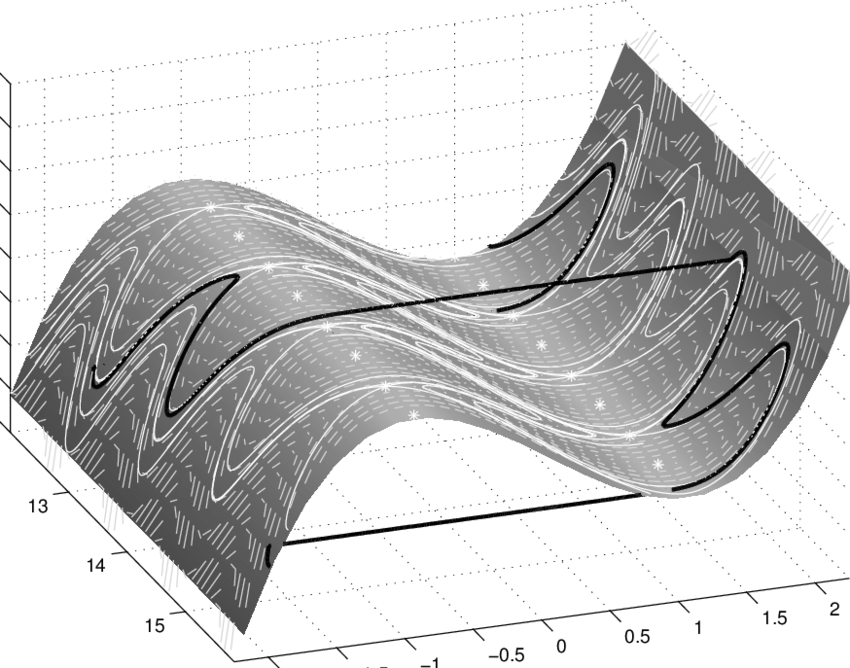
\includegraphics[height=10cm,width=14cm]{Images/Three-dimensional-plot-of-a-trajectory-for-the-van-der-Pol-equation-and-the-critical}
	\caption{Three dimensional \vdp \citep{3D-VdP}.}
	\label{fig: 3d folded singularity}
\end{figure}\newpage
as our fold point now can take multiple locations within our system, denoted by `*'. From here we are able to define some non-degeneracy conditions, much like we did in Section \ref{GSPT},
\begin{equation}
\begin{aligned}
&f(p_*,\lambda,0)=0,\\
&\pd{}{x}f(p_*,\lambda,0)=0,\\
&\pd{^2}{x^2}f(p_*,\lambda,0)\neq 0,\\
&D_{(y,z)}f(p_*,\lambda,0) \ \text{has full rank one},
\end{aligned}
\label{eq: non-degeneracy 3d system}	
\end{equation}
where we denote $ p_*=(x_*,y_*,z_*)\in F $ as our fold points and\textbf{ $ D_{(y,z)}=(\pd{f}{y},\pd{f}{z}) $ are linearly independent of one another } \citep{MMO}. In addition to this we can see from Figure \ref{fig: 3d folded singularity} that we have some interesting flows within our system. These flows do not follow the standard pattern as we saw in Figure \ref{fig: vdp flow diagram}, instead the slow flow switches its orientation when the flow hits the fold point and continue to flow in that direction, as a desingularised flow - these are called isolated singularities \citep{MMO}.+++just say folded singularity, consider reduced system. folded sing. is equ.. of reduced system... introduce folded line...++ aiming to find x equn as before for reduced flow, desingularise by time and move on++
 %dot in diagram
%As a result we are able to express these flows in the following manner, using Equation \ref{eq: non-degeneracy 3d system}, 
As a result we are able to write these flows in the following manner, using Equations \ref{eq: fs singularity system}, \ref{eq: non-degeneracy 3d system} and noting that $ \od{x}{t}=0=\pd{f}{x} $,  
\begin{equation}
-\pd{f}{x}x'=y'\pd{f}{y}+z'\pd{f}{z},
\end{equation}
where we can note that $ y'=g_1 $ and $ z'=g_2 $. We then make a scaling in time \st $ t=-\pd{f}{x} $ wto give the system in the desired form,\\

%$\frac{\dif x}{\dif t} = \frac{\dif y}{\dif t} \frac{\partial f}{\partial y} +  \frac{\dif z}{\dif t} \frac{\partial f}{\partial z}$

\begin{equation} \label{somegenericthreedim}
\begin{cases}
\dot{x}&=g_1\pd{f}{y}+g_2\pd{f}{z},\\
\dot{y}&=-g_1\pd{f}{x},\\
\dot{z}&=-g_2\pd{f}{x}.
\end{cases}
\end{equation}
From here we can then define a folded singularity if $ g_1(p_*,\lambda,0)\pd{}{y}f(p_*,\lambda,0)+g_2(p_*,\lambda,0)\pd{}{z}f(p_*,\lambda,0)=0 $, for our flow on branches ($ S $) \citep{MMO}. Next we need to consider the stability of our fold points. We do this by constructing the Jacobian of our system, 
\begin{equation}
J=\begin{bmatrix}
\pd{\dot{x}}{x}&\pd{\dot{x}}{y}&\pd{\dot{x}}{z}\\
\pd{\dot{y}}{x}&\pd{\dot{y}}{y}&\pd{\dot{y}}{z}\\
\pd{\dot{z}}{x}&\pd{\dot{z}}{y}&\pd{\dot{z}}{z}\\
\end{bmatrix},
\end{equation}

which we can easily find the eigenvalues, by taking the determinant. The result of this analysis gives that we have three eigenvalues, $ \sigma_i $ for $ i=1,2,3 $ \citep{MMO}. \Wlg we can choose $ \sigma_3=0 $ because we know that at least one of our eigenvalues must be zero to account for our fold point in our system.
++++call it classification of...++++
 Then we know from standard stability theory that, at our folded singularity we will have three types of phase portrait in the form of,
\begin{equation}
\begin{cases}
Saddle \ \sigma_1\sigma_2<0: \sigma_i\in\Re,\\
Node \ \sigma_1\sigma_2>0: \sigma_i\in\Re,\\
Focus \ \sigma_1\sigma_2>0: \Im(\sigma_i)\neq 0,
\end{cases}
\end{equation}
where we can note that only our focus will have imaginary parts \citep{MMO}. \citet{MMO} illustrates this in the following Figure, 
\begin{figure}[h!]\centering
	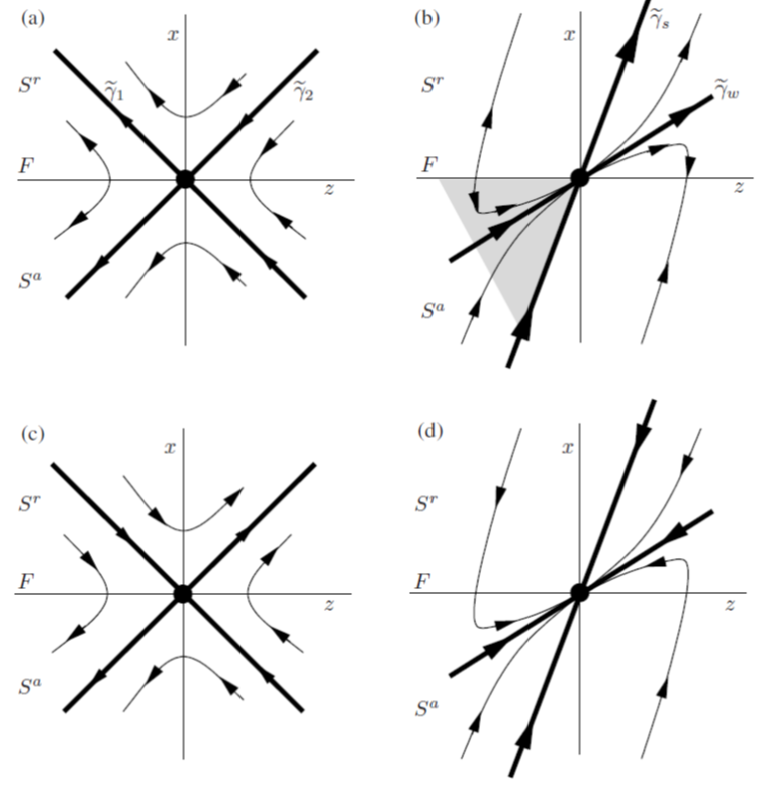
\includegraphics[height=12cm,width=12cm]{Images/foldednodesetc}
	\caption{Phase portraits of our three dimensional system where a) is a folded saddle, b) folded node, c) and d) are desingularised flows \citep{MMO}.}
	\label{fig: folded singularities}
\end{figure}\newpage%arrows switch as we have reversed time
where we can see the effect of the varying eigenvalues above. A question which is prudent to consider is, why has not \citep{MMO} illustrated the singular canard case for a folded focus. This is easily answered as we know that a singular canard is only present if the node or saddle connect our two connecting branches ($ S^r $ and $ S^a $). The idea that our branches are connected allows us to note that our flow is able to pass through from an attracting to a repelling manifold, which is described by Figure \ref{fig: folded singularities} \citep{CanardsinR3}. 
\begin{figure}[h!]\centering
	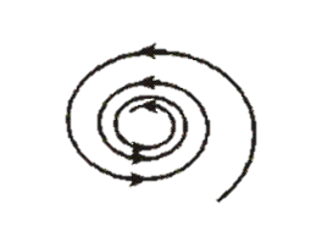
\includegraphics{Images/spiral3}
	\caption{The branches of a spiral \citep{Spiral}.}
	\label{fig: spiral}
\end{figure}\newpage
However, we find that for the focus we are unable to construct branches which connect, preventing the flow from traversing through the fold point. This idea is easily seen as we are able to note, from the imaginary eigenvalues, that there is a spiral present - Figure \ref{fig: spiral}.
It is easily seen, from Figure \ref{fig: spiral}, that it is not possible to construct such a system that allows the flow to traverse this point for the folded focus. We can add further intuition to this example by considering the notion of a source (or sink), which is seen in dynamical systems and fluid mechanics. From a sink (attracting manifold) we know that our flow will always be travelling towards the singularity regardless of its starting location as described by Figure \ref{fig: spiral} meaning that is impossible to construct a repelling manifold which can connect with this singularity at the fold point.

\begin{theorem}[Canards in $ \Re^3 $ \citep{MMO}]\label{thm: canards in R3}
	For slow-fast systems (Equation \ref{eq: fs singularity system}) with $ \epsilon>0 $ sufficiently small the following holds:\begin{itemize} 
		\item  There are no maximal canards generated by a folded focus. For a folded saddle the two singular canards $ \bar{\gamma_{1,2}} $ perturb to maximaal canards $ \gamma_{1,2} $.
		\item  For a folded node let $\mu=\frac{\sigma_w}{\sigma_s} <1$. the singular canard $ \bar{\gamma_{s}} $ (``the strong canard'') always perturbs to a maximal canard $ \gamma_{s} $. If $ \mu^{-1}\not \in \mathbb{N} $, then the singualr canard $ \bar{\gamma_{w}} $ (``weak canard'') also perturbs to a maximal canard. We call $ \gamma_{s} $ and $ \gamma_{w} $ primary canards.
		\item For a folded node suppose $ k>0 $ is an integer such that $ 2k+1<\mu^{-1} <2k+3$ and $ \mu^-1\neq 2(k+1) $. Then, in addition to $ \gamma_{s,w} $ there are k other maximal canards, which we call secondary canard.
		\item The primary weak canard of a node undergoes a trancritical bifurcation for odd $ \mu^{-1}\in\mathbb{N} $ and a pitchfork bifurcation for even $ \mu^{-1}\in\mathbb{N} $
	\end{itemize}
	\end{theorem}
From Theorem \ref{thm: canards in R3} we have now defined the existence of a strong and weak eigenvalue \st $ |\sigma_1|>|\sigma_2| \iff |\sigma_s|>|\sigma_w| $. From this theorem we are then able to carry out explicit investigations, as we will see in Section \textbf{Not done yet} noting that a focus is a circle or spiral etc.
++++ add comments about if $\mu $ is natural, bifurcations, refer to wechselberger, explain weak and strong eigenvalues, explain the singular canards (definition!)++++
make note that we can desingularise, rescale and blow up to investigate......

desingularizing by changing the top half plane for arrows 






















\subsection{ The Folded Node}
In this section the occurence of different SAOs due to a folded node of the reduced system is discussed and conditions for a global return mechanism, which gives rise to MMOs, are presented.
The folded node singularity is an equilibrium of the reduced system. Note that it is only defined on $S$, the critical manifold and therefore only for the slow flow. There is no global equilibrium, wich will become apparent in this section.
The normal form considered for analysing the folded node singularity is in terms of the space variables $(u,v,w)$, and given by:

\begin{align*}
\epsilon \dot{u} &= v - u^2\\
\dot{v} &= w-u\\
\dot{w} &= - \nu
\end{align*}

Then the system can be transformed using the following coordinate and time transformation:
\begin{align}\label{normalform1}
u= \frac{x}{(1+ \mu)^{1/2}}, \ \ \ v &= \frac{y}{(1 + \mu)}, \ \ \  w= -\frac{z}{ (1+\mu)^{3/2}}  \\
\tau &= \frac{\tau_1}{\sqrt{1 + \mu}},
\end{align}
where $\tau_1$ is the original time variable and $\tau$ is the transformed time variable.
Then $\frac{d \tau}{d \tau_1} = \frac{1}{\sqrt{1+ \mu}}$, and the system becomes:
\begin{align}\label{normalform2}
\epsilon \dot{x} &= y - x^2\\
\dot{y} &=- z -(\mu +1)x \\
\dot{z} &= \nu (1 + \mu)^2
\end{align}
where $\mu$ is the eigenvalue ratio from before.
This is nearly in the form presented in \citet{MMO}, however, the $z$ equation there is witten purely in terms of $\mu$ as $\dot{z} = \frac{1}{2} \mu$.
Equating these two representations yields a relationship between $\mu$ and $\nu$:
\begin{align*}
&\nu (1 + \mu)^2 = \frac{1}{2} \mu \\
&\Rightarrow \nu = \frac{\mu}{ 2 (1+ \mu)^2},
\end{align*}
and this is equivalent to 
\begin{align*}
\mu = \frac{ -1 + \sqrt{1 - 8\nu}}{-1 - \sqrt{ 1- 8 \nu}},
\end{align*}
since $0< \mu < 1$ and $\mu \in \mathbf{R}$. (++++ unsure about reasoning+++)

Note here that the reason that no global equilibrium exists is because \ref{normalform1} can only have an equilibrium if $\dot{w} =0$. This would imply that $\nu=0$, however, as the previous calculations have shown, $\nu$ is dependent on the eigenvalue ratio $\mu$. Since $\mu \neq 0$ for the folded node, as will be demonstrated below, $\nu$ cannot be zero.
It is now of interest to verify the location of the folded singularity at the origin, and therefore derive the reduced system as well as the eigenvalues for the reduced problem.
Consider equation (\ref{normalform2}) and define $\dot{x}:=f$ as before. The reduced problem, as $\epsilon \to 0$ becomes $f= y-x^2 =0$, and therefore the critical manifold is defined as $S:= \{ (x,y,z) : y=x^2\}$, which is an S shaped two dimensional plane.
Now that $f$ is defined explicitly, we can check the nondeceneracy conditions for a folded singularity, as presented in (\ref{eq: non-degeneracy 3d system}) and get the follwing results:
\begin{align*}
&f(x,y,z,,\mu, \epsilon) = 0\\
&\Rightarrow y=x^2\\
\\
&\frac{\partial f}{\partial x} (x,y,z,\mu,\epsilon) = 2x = 0\\
&\Rightarrow x=0 \Rightarrow y=0 \\ 
&\frac{\partial^2 f}{\partial x^2}(x,y,z,\mu,\epsilon)  = 2 \neq 0\\
&D_{(y,z)}f= (1,0) \textrm{ full rank one}.
\end{align*}
This shows that there exists a fold line $L:=(0,0,z)$ on the slow manifold $S$.
In order to determine at which value of $z$ the folded node singularity is located, we have to consider the reduced system of (\ref{normalform2}), where we replace $\nu (1 + \mu)^2$ with $\frac{1}{2} \mu$ for convenience. The aim is to find an equilibrium of the reduced problem, since we know from the theory discussed that the folded singularity is an equilibrium of the slow flow.
The reduced problem is:
\begin{align}\label{normalform2red}
0 &= y - x^2 :=f\\
\dot{y} &=- z -(\mu +1)x \\
\dot{z} &=\frac{1}{2} \mu 
\end{align}
Therefore, the slow flow is derived, analogous to Section (I+++ i guess VDP but also after that+++). 
First, the equation $f=0$ is considered and it is noted that we can take the derivative with respect to the time variable to get 
\begin{align} \label{yxderivrel}
\dot{y} = 2x \dot{x},
\end{align}
 and this can be rearranged to give an expression for the dynamics in $x$ on the slow manifold:
\begin{align*}
\dot{x}= \frac{\dot{y}}{2x},
\end{align*}
which is singular for $x=0$, which coinsides with the fold line.
This expression can be desingularised by rescaling time in the whole reduced system by a factor of $2x$. This results in
\begin{align} \label{fullredsysformmo}
&\dot{x} = -(\mu+1)x - z \notag \\
&\dot{y} = - 2x (\mu +1) -2xz\\
&\dot{z} = x \mu \notag,
\end{align}
however, it can be noted that the equation for $y$ can be ommited, since the change in $y$ is directly related to the change in $x$ by a factor of $2x$ as stated in equation (\ref{yxderivrel})(+++mention CMT?+++). Therefore, the reduced dynamics can be sufficiently described by
\begin{align}\label{twovarxzred}
&\dot{x} = -(\mu+1)x - z\\
&\dot{z} = x \mu. \notag
\end{align}
Now, following the theory for folded singularities, the folded node has to satisfy the condition (+++add name of the condition and generalized statement of it+++)
\begin{align*}
& -(\mu+1)x - z=0 |_{(0,0,z)}\\
&\Rightarrow z=0,
\end{align*}
which leads to the conclusion that the folded singularity, defined on the slow manifold for $\epsilon \to 0$ and located on the fold line $L=(0,0,z)$, is given by $(0,0,0)$, as expected.
The next step of the analysis is to verify that the folded singularity at the origin is indeed a folded node.
As discussed in Section \ref{sec: threedimfolds}, the classification of the singularities is determined by the eigenvalues of the reduced system. Therefore, the next step is calculating these eigenvalues.
The Jacobian of the reduced system (\ref{twovarxzred}) is
\begin{equation}
J=\begin{bmatrix}
-(\mu +1) & -1 \\
\mu & 0 \\
\end{bmatrix},
\end{equation}
and therefore the characteristic equation yields
\begin{align*}
&\sigma^2 +(\mu +1)\sigma + \mu = 0 \\
&\Rightarrow \sigma_1= -1 \textrm{\ \ \ and \ \ \ } \sigma_2 = -\mu.
\end{align*}
Since $\mu$ is the eigenvalue ratio and satisfies $0< \mu < 1$, we can conclude that 
\begin{align*}
\sigma_1\sigma_2 = (-1)(-\mu)=\mu >0,
\end{align*}
and therefore, by the conditions presented in Section \ref{sec: threedimfolds}, this shows that the folded singularity is in fact a folded node.
Note that if we had tried to find the eigenvalues for the full three dimensional reduced system (\ref{fullredsysformmo}) instead, an additional eigenvalue $\sigma_3=0$ would have occured. This is the eigenvalue that corresponds to the loss of hyperbolicity at the folded node, which is expected for singular points.

In order to analyse the folded node, the system (\ref{normalform1}) is transformed using the blow up transformation $u= \epsilon^{1/2}\overline{x}, v=\epsilon \overline{y}, w= \epsilon^{1/2} \overline{z}$ and $ \tau_1 = \epsilon^{1/2} \overline{t}$.
Then, in a neighbourhood $U$ of the folded node the system is represented by
\begin{align*}
\dot{\overline{x}}= \overline{y} - \overline{x}^2\\
\dot{\overline{y}}=\overline{z} - \overline{x} \\
\dot{\overline{z}}= - \nu.
\end{align*}
In the following analysis, the bars will be omitted for readability.
One important realisation is that the phase portraits for the rescaled system is topologically equivalent to the original normal form. Therefore, the mapping of solutions  found in the blown up system to the original system is straightforward. ++++check if true++++

All the information needed to describe the dynamics near the fold point is now derived and therefore the next step in the analysis is the descripton of the SAOs. The SAOs in the folded node case are candard trajectories that follow a certain pattern.
These patterns are, as discussed in Theorem \ref{thm: canards in R3}, found by considering the eigenvalue ratio $\mu$.
In the case of the folded node, $\mu$ satisfies $2k+1 < \mu^{-1} < 2k +3 $. Solving for $k \in \mathbf{N}$, then $k$ is the number of secondary canards in the system as stated in Theorem \ref{thm: canards in R3}. Furthermore, $k$ corresponds to the number of twists the primary canard $\gamma_s$ is performing around $\gamma_w$. A twist corresponds to a $180^{\circ}$ rotation, see \citet{kuehn}. It is important to note that $\mu^{-1} \notin \mathbf{N}$ in order to conclude the number of secondary canards.
If $\mu^{-1} \in \mathbf{N}$ 

These SAOs are happening when trajectories get funneled into the region of the fold and contracted along the direction of $S^a$(+++++?????++++). For different values of $\epsilon$, the funnel gets narrower. For $\epsilon \to 0$, the maximum canard basically coinsides with all of them... or something like that....
The number of SAOs an incoming trajectory undergoes depends on where the trajectory enters the fold region in the $z$ plane. Different intervals of $z$ can be defined in order to indicate for which values of $z$ a certain amount of SAOs will be observed. The intervals are not 'clear cut', and a mix can happen +++??+++
The interval for the primary strong canard is significantly larger, so the secondary canards close to it will have a higher amplitude (? reasoning right?) while the number of SAOs is smaller. As the number of SAOs increases, the amplitude of oscillations get smaller (contraction ?) and are not readily visible.
The result about the width of the intervals is summed up in the following theorem.

\begin{theorem}[\textbf{Width of Rotational Sectors}][\citealp{MMO}]
Consider system (\ref{somegenericthreedim}) and assume it has a folded-node singularity. At an $O(1)$ distance from the fold curve, all secondary canards are in an $O(\epsilon^{(1- \mu)/2)})$ neighbourhood of the primary strong canard. Hence, the width of the  rotational sectors $I_i, 1 \leq i \leq k$, is $O(\epsilon^{(1- \mu)/2)})$ and the width of sector $I_{k+1}$ is $O(1)$.
\end{theorem}



